\documentclass{article}\usepackage[]{graphicx}\usepackage[]{color}
%% maxwidth is the original width if it is less than linewidth
%% otherwise use linewidth (to make sure the graphics do not exceed the margin)
\makeatletter
\def\maxwidth{ %
  \ifdim\Gin@nat@width>\linewidth
    \linewidth
  \else
    \Gin@nat@width
  \fi
}
\makeatother

\definecolor{fgcolor}{rgb}{0.345, 0.345, 0.345}
\newcommand{\hlnum}[1]{\textcolor[rgb]{0.686,0.059,0.569}{#1}}%
\newcommand{\hlstr}[1]{\textcolor[rgb]{0.192,0.494,0.8}{#1}}%
\newcommand{\hlcom}[1]{\textcolor[rgb]{0.678,0.584,0.686}{\textit{#1}}}%
\newcommand{\hlopt}[1]{\textcolor[rgb]{0,0,0}{#1}}%
\newcommand{\hlstd}[1]{\textcolor[rgb]{0.345,0.345,0.345}{#1}}%
\newcommand{\hlkwa}[1]{\textcolor[rgb]{0.161,0.373,0.58}{\textbf{#1}}}%
\newcommand{\hlkwb}[1]{\textcolor[rgb]{0.69,0.353,0.396}{#1}}%
\newcommand{\hlkwc}[1]{\textcolor[rgb]{0.333,0.667,0.333}{#1}}%
\newcommand{\hlkwd}[1]{\textcolor[rgb]{0.737,0.353,0.396}{\textbf{#1}}}%
\let\hlipl\hlkwb

\usepackage{framed}
\makeatletter
\newenvironment{kframe}{%
 \def\at@end@of@kframe{}%
 \ifinner\ifhmode%
  \def\at@end@of@kframe{\end{minipage}}%
  \begin{minipage}{\columnwidth}%
 \fi\fi%
 \def\FrameCommand##1{\hskip\@totalleftmargin \hskip-\fboxsep
 \colorbox{shadecolor}{##1}\hskip-\fboxsep
     % There is no \\@totalrightmargin, so:
     \hskip-\linewidth \hskip-\@totalleftmargin \hskip\columnwidth}%
 \MakeFramed {\advance\hsize-\width
   \@totalleftmargin\z@ \linewidth\hsize
   \@setminipage}}%
 {\par\unskip\endMakeFramed%
 \at@end@of@kframe}
\makeatother

\definecolor{shadecolor}{rgb}{.97, .97, .97}
\definecolor{messagecolor}{rgb}{0, 0, 0}
\definecolor{warningcolor}{rgb}{1, 0, 1}
\definecolor{errorcolor}{rgb}{1, 0, 0}
\newenvironment{knitrout}{}{} % an empty environment to be redefined in TeX

\usepackage{alltt}
\usepackage{natbib}
\usepackage[unicode=true]{hyperref}
\usepackage{geometry}
\geometry{tmargin=1in,bmargin=1in,lmargin=1in,rmargin=1in}


\IfFileExists{upquote.sty}{\usepackage{upquote}}{}
\begin{document} 
\title{STAT243-PS3}
\author{Jinhui Xu}
\date{September 2017}

\maketitle

\section{Other students}
I discuss some problems with Xin Shi.  

\section{Question 1}
Material four : Millman and Perez\\

The article emphasizes the importance of good practice of computational work. It first introduces its vision for scientific software development in everyday research. Then gives specific recommendations for computational work.\\

I think the article is meaningful. As when I was confused about my project thesis, I would search solutions on the internet. However, the code I found usually did not work because I did not know how to use the data and which tools should I use. Therefore I think that good practice of computational work is necessary.\\

The article gives recommendations on each step of research work from initial exploration of ideas and data to final results,including Individual exploration,  Collaboration, Production-scale execution, Publication and Education.\\


But I am not familiar with some tools and process the article mentions, so I have two questions:\\

Q1: the article says that the Python language has a simple, expressive, and accessible syntax that emphasizes code readability. I don’t know what code readability means? Whether R or other languages do well in code readability?\\

Q2: In the section of collaboration, the article mentions the concept of distributed version control systems. Are Mercurial or other DVCS similar with git? Whether git is enough for us?

\section{Question 2}
 
\subsection{(a)}

In this section, I add each play into a list which call playlist. As at the begin of each play, there is year of play, so I grep the str start with four digits and get 38 years. Delete the first one and the last one, I can obtain plays by reading the content between two years.
\begin{knitrout}
\definecolor{shadecolor}{rgb}{0.969, 0.969, 0.969}\color{fgcolor}\begin{kframe}
\begin{alltt}
\hlcom{#read the original txt and store it in text}
\hlstd{text}\hlkwb{=}\hlkwd{readLines}\hlstd{(}\hlstr{"http://www.gutenberg.org/cache/epub/100/pg100.txt"}\hlstd{)}
\hlcom{#get rownumber of year in text and store 36 years in vector year_play,it is for question (b)}
\hlstd{year_rownumber}\hlkwb{=}\hlkwd{grep}\hlstd{(}\hlstr{'^[[:digit:]]\{4\}'}\hlstd{,text)}
\hlstd{year_play}\hlkwb{=}\hlstd{text[year_rownumber[}\hlnum{2}\hlopt{:}\hlstd{(}\hlkwd{length}\hlstd{(year_rownumber)}\hlopt{-}\hlnum{1}\hlstd{)]]}
\hlcom{#store each play in playlist,I believe that the content between year of play_i }
\hlcom{#and year of play_i+1 is exactly the content of play_i}
\hlstd{playlist}\hlkwb{=}\hlkwd{list}\hlstd{()}
\hlkwa{for}\hlstd{(i} \hlkwa{in} \hlnum{1}\hlopt{:}\hlnum{36}\hlstd{) playlist[[i]]}\hlkwb{=}\hlstd{text[(year_rownumber[i}\hlopt{+}\hlnum{1}\hlstd{])}\hlopt{:}\hlstd{(year_rownumber[i}\hlopt{+}\hlnum{2}\hlstd{]}\hlopt{-}\hlnum{1}\hlstd{)]}
\end{alltt}
\end{kframe}
\end{knitrout}

\subsection{(b)}

I have get year\_play in Q(a), and get the title of play by obtaining content in the second row (not NULL) of a play.
The way to get the number of acts and the number of scenes is similar so I write a function named count\_number(str\_target,searchlist).str\_target is a regex to be matched in searchlist. And the output is a list contain content\_list and count\_number.
\begin{knitrout}
\definecolor{shadecolor}{rgb}{0.969, 0.969, 0.969}\color{fgcolor}\begin{kframe}
\begin{alltt}
\hlcom{#the second row is exactly the title of play.}
\hlstd{title}\hlkwb{=}\hlkwd{c}\hlstd{();}
\hlkwa{for}\hlstd{(i} \hlkwa{in} \hlnum{1}\hlopt{:}\hlnum{36}\hlstd{) title[i]}\hlkwb{=}\hlstd{playlist[[i]][}\hlkwd{which}\hlstd{(playlist[[i]]}\hlopt{!=}\hlstr{""}\hlstd{)[}\hlnum{2}\hlstd{]]}
\hlcom{#get the number of scenes by locate the str , and the number of acts equels to the number of unique name of act ,}
\hlcom{#the function to get the number of acts and scenes}
\hlkwd{library}\hlstd{(stringr)}
\hlstd{count_number}\hlkwb{=}\hlkwa{function}\hlstd{(}\hlkwc{str_target}\hlstd{,}\hlkwc{searchlist}\hlstd{)\{}
  \hlstd{content_list}\hlkwb{=}\hlkwd{list}\hlstd{()}
  \hlstd{content_number}\hlkwb{=}\hlkwd{c}\hlstd{()}
  \hlkwa{for}\hlstd{(i} \hlkwa{in} \hlnum{1}\hlopt{:}\hlkwd{length}\hlstd{(searchlist))\{}
    \hlstd{str_locate}\hlkwb{=}\hlkwd{c}\hlstd{()}
    \hlstd{str_locate}\hlkwb{=}\hlkwd{grep}\hlstd{(str_target,searchlist[[i]])}
    \hlstd{content_list[[i]]}\hlkwb{=}\hlstd{searchlist[[i]][str_locate]}
    \hlstd{content_number[i]}\hlkwb{=}\hlkwd{length}\hlstd{(str_locate)}
  \hlstd{\}}
  \hlstd{list}\hlkwb{=}\hlkwd{list}\hlstd{(content_list,content_number)}
  \hlkwd{return}\hlstd{(list)}
\hlstd{\}}
\end{alltt}
\end{kframe}
\end{knitrout}
Run the function to get  act\_number and scene\_number
\begin{knitrout}
\definecolor{shadecolor}{rgb}{0.969, 0.969, 0.969}\color{fgcolor}\begin{kframe}
\begin{alltt}
\hlstd{scene_list}\hlkwb{=}\hlkwd{list}\hlstd{();act_list}\hlkwb{=}\hlkwd{list}\hlstd{();scene_number}\hlkwb{=}\hlkwd{c}\hlstd{();act_number}\hlkwb{=}\hlkwd{c}\hlstd{()}
\hlstd{scene_str}\hlkwb{=}\hlstr{"[S][Cc][Ee][Nn][Ee][[:blank:]]"}
\hlstd{act_str}\hlkwb{=}\hlstr{"A[Cc][Tt] "}
\hlstd{scene_list}\hlkwb{=}\hlkwd{count_number}\hlstd{(scene_str,playlist)[[}\hlnum{1}\hlstd{]]}
\hlstd{scene_number}\hlkwb{=}\hlkwd{count_number}\hlstd{(scene_str,playlist)[[}\hlnum{2}\hlstd{]]}
\hlstd{act_list}\hlkwb{=}\hlkwd{count_number}\hlstd{(act_str,playlist)[[}\hlnum{1}\hlstd{]]}
\hlstd{act_number}\hlkwb{=}\hlkwd{c}\hlstd{();}\hlkwa{for}\hlstd{(i} \hlkwa{in} \hlnum{1}\hlopt{:} \hlnum{36}\hlstd{) act_number[i]}\hlkwb{=}\hlkwd{length}\hlstd{(}\hlkwd{unique}\hlstd{(}\hlkwd{str_extract_all}\hlstd{(act_list[[i]],}
\hlstr{'A[Cc][Tt][[:blank:]]?[[:alpha:]]*'}\hlstd{)))}
\end{alltt}
\end{kframe}
\end{knitrout}

Then extract the body and store five factors in a list. the information of play\_i is stored in result{[[i]]}
\begin{knitrout}
\definecolor{shadecolor}{rgb}{0.969, 0.969, 0.969}\color{fgcolor}\begin{kframe}
\begin{alltt}
\hlstd{body_list}\hlkwb{=}\hlkwd{list}\hlstd{();}
\hlkwa{for}\hlstd{(i} \hlkwa{in} \hlnum{1}\hlopt{:}\hlnum{36}\hlstd{) body_list[[i]]}\hlkwb{=}\hlstd{playlist[[i]][}\hlkwd{grep}\hlstd{(}\hlstr{"^[[:blank:]]*[Ss][Cc][Ee][Nn][Ee][[:punct:]]"}
\hlstd{,playlist[[i]])}\hlopt{:}\hlkwd{length}\hlstd{(playlist[[i]])]}
\hlstd{result}\hlkwb{=}\hlkwd{list}\hlstd{()}
\hlkwa{for}\hlstd{(i} \hlkwa{in} \hlnum{1}\hlopt{:}\hlnum{36}\hlstd{) \{}
  \hlstd{play_result}\hlkwb{=}\hlkwd{list}\hlstd{()}
  \hlstd{play_result[[}\hlnum{1}\hlstd{]]}\hlkwb{=}\hlstd{year_play[i]}
  \hlstd{play_result[[}\hlnum{2}\hlstd{]]}\hlkwb{=}\hlstd{title[i]}
  \hlstd{play_result[[}\hlnum{3}\hlstd{]]}\hlkwb{=}\hlstd{act_number[i]}
  \hlstd{play_result[[}\hlnum{4}\hlstd{]]}\hlkwb{=}\hlstd{scene_number[i]}
  \hlstd{play_result[[}\hlnum{5}\hlstd{]]}\hlkwb{=}\hlstd{body_list[[i]]}
  \hlkwd{names}\hlstd{(play_result)}\hlkwb{=}\hlkwd{c}\hlstd{(}\hlstr{'year'}\hlstd{,}\hlstr{'title'}\hlstd{,}\hlstr{'number of acts'}\hlstd{,}\hlstr{'number of scenes'}\hlstd{,}\hlstr{'body'}\hlstd{)}
  \hlstd{result[[i]]}\hlkwb{=}\hlstd{play_result}
\hlstd{\}}
\end{alltt}
\end{kframe}
\end{knitrout}

view the result of play\_1 except the body of play (too large)
\begin{knitrout}
\definecolor{shadecolor}{rgb}{0.969, 0.969, 0.969}\color{fgcolor}\begin{kframe}
\begin{alltt}
\hlstd{result[[}\hlnum{1}\hlstd{]]}\hlopt{$}\hlstd{year}
\end{alltt}
\begin{verbatim}
## [1] "1603"
\end{verbatim}
\begin{alltt}
\hlstd{result[[}\hlnum{1}\hlstd{]]}\hlopt{$}\hlstd{title}
\end{alltt}
\begin{verbatim}
## [1] "ALLS WELL THAT ENDS WELL"
\end{verbatim}
\begin{alltt}
\hlstd{result[[}\hlnum{1}\hlstd{]]}\hlopt{$}\hlstr{'number of acts'}
\end{alltt}
\begin{verbatim}
## [1] 5
\end{verbatim}
\begin{alltt}
\hlstd{result[[}\hlnum{1}\hlstd{]]}\hlopt{$}\hlstr{'number of scenes'}
\end{alltt}
\begin{verbatim}
## [1] 23
\end{verbatim}
\end{kframe}
\end{knitrout}

\subsection{(c)}

First,update the body\_list,delete the first 5 rows of body. I suppose that part of information are confused.
\begin{knitrout}
\definecolor{shadecolor}{rgb}{0.969, 0.969, 0.969}\color{fgcolor}\begin{kframe}
\begin{alltt}
\hlstd{body_update}\hlkwb{=}\hlstd{body_list}
\hlkwd{library}\hlstd{(stringr)}
\hlkwa{for}\hlstd{(i} \hlkwa{in} \hlnum{1}\hlopt{:}\hlnum{36}\hlstd{)\{}
  \hlstd{n}\hlkwb{=}\hlkwd{grep}\hlstd{(}\hlstr{"[S][Cc][Ee][Nn][Ee][[:blank:]]"}\hlstd{,body_list[[i]])}
  \hlkwa{for}\hlstd{(j} \hlkwa{in} \hlnum{1}\hlopt{:}\hlkwd{length}\hlstd{(n))}
  \hlstd{body_update[[i]][n[j]}\hlopt{:}\hlstd{(n[j]}\hlopt{+}\hlnum{4}\hlstd{)]}\hlkwb{=}\hlstr{'null'}
\hlstd{\}}
\end{alltt}
\end{kframe}
\end{knitrout}

get the unique speaker name.I suppose that every speaker's name begins with a upper,every chunk must have at least one lower.
\begin{knitrout}
\definecolor{shadecolor}{rgb}{0.969, 0.969, 0.969}\color{fgcolor}\begin{kframe}
\begin{alltt}
\hlstd{speaker_first_content}\hlkwb{=}\hlkwd{list}\hlstd{()}
\hlstd{name}\hlkwb{=}\hlkwd{list}\hlstd{()}
\hlstd{speaker_locate}\hlkwb{=}\hlkwd{list}\hlstd{()}
\hlstd{speaker_number}\hlkwb{=}\hlkwd{c}\hlstd{()}
\hlkwa{for}\hlstd{(i} \hlkwa{in} \hlnum{1}\hlopt{:}\hlnum{36}\hlstd{)\{}

\hlcom{#delete several specific stage direction like Exit,Enter...}
  \hlstd{body_update[[i]]}\hlkwb{=}\hlkwd{str_replace_all}\hlstd{(body_update[[i]],}\hlstr{'((Exit|Exeunt|Enter|Re-enter)([[:graph:]
[:blank:]])*)|(\textbackslash{}\textbackslash{}[([[:graph:][:blank:]])+\textbackslash{}\textbackslash{}])'}\hlstd{,}\hlstr{''}\hlstd{)}

\hlcom{#find the sentences that begin with a speaker's name plus [.]}
  \hlstd{speaker_locate[[i]]}\hlkwb{=}\hlkwd{grep}\hlstd{(}\hlstr{'^[[:blank:]]\{0,4\}[[:upper:]]+[[:lower:]]*([[:blank:]]*[[:upper:]]+
[[:lower:]]*)*[.][[:blank:]]*[[:upper:]][[:blank:]]*[[:punct:]]*([[:blank:]][[:upper:]])?[[:blank:]]*
[[:punct:]]?[[:lower:]]'}\hlstd{,body_update[[i]])}
  \hlstd{speaker_first_content[[i]]}\hlkwb{=}\hlstd{body_update[[i]][speaker_locate[[i]]]}

\hlcom{#group each speaker's names in to list of name.and delete trashy blanks}
  \hlstd{name[[i]]}\hlkwb{=}\hlkwd{unique}\hlstd{(}\hlkwd{str_replace_all}\hlstd{(}\hlkwd{str_extract}\hlstd{(speaker_first_content[[i]],}\hlstr{"^[[:blank:]]\{0,4\}
[[:upper:]]+[[:lower:]]*([[:blank:]]*[[:upper:]]*[[:lower:]]*)\{0,2\}"}\hlstd{),}\hlstr{"^[[:blank:]]*"}\hlstd{,}\hlstr{''}\hlstd{))}

\hlcom{#I suppose that  play's names are either all upper cases or all lower cases except the first one. }
\hlcom{#So find plays whose names are all upper cases and delete confused 'names' that contains lower cases. }
  \hlkwa{if}\hlstd{((}\hlkwd{length}\hlstd{(}\hlkwd{grep}\hlstd{(}\hlstr{'[[:lower:]]+'}\hlstd{,name[[i]]))}\hlopt{/}\hlkwd{length}\hlstd{(name[[i]]))}\hlopt{<}\hlnum{0.3}\hlopt{&&}\hlstd{(}\hlkwd{length}\hlstd{(}\hlkwd{grep}\hlstd{(}\hlstr{'[[:lower:]]+'}\hlstd{,}
\hlstd{name[[i]]))}\hlopt{/}\hlkwd{length}\hlstd{(name[[i]]))}\hlopt{>}\hlnum{0}\hlstd{)             name[[i]]}\hlkwb{=}\hlstd{name[[i]][}\hlopt{-}\hlkwd{grep}\hlstd{(}\hlstr{'[[:lower:]]+'}\hlstd{,name[[i]])]}

\hlcom{#calculate the number of unique speakers required in Q(d)}
  \hlstd{speaker_number[i]}\hlkwb{=}\hlkwd{length}\hlstd{(name[[i]])}
\hlstd{\}}
\end{alltt}
\end{kframe}
\end{knitrout}
Store all information of chunks in a list called chunk\_name\_play. chunk\_name\_play{[[i]]} contains all all chunks of each speaker in play\_i, and chunk\_name\_play{[[i]][[j]]} contains all chunks of speaker\_j in play\_i. 
\begin{knitrout}
\definecolor{shadecolor}{rgb}{0.969, 0.969, 0.969}\color{fgcolor}\begin{kframe}
\begin{alltt}
\hlstd{chunk_name_play}\hlkwb{=}\hlkwd{list}\hlstd{();}
\hlkwa{for}\hlstd{(r} \hlkwa{in} \hlnum{1}\hlopt{:}\hlnum{36}\hlstd{)\{}
  \hlstd{chunk}\hlkwb{=}\hlkwd{list}\hlstd{();}\hlkwa{for}\hlstd{(k} \hlkwa{in} \hlnum{1}\hlopt{:}\hlkwd{length}\hlstd{(name[[r]]))\{}
     \hlcom{# in play_r,get the location of speakers_k'names,store them in vector l}
     \hlstd{l}\hlkwb{=}\hlkwd{c}\hlstd{()}
     \hlstd{l}\hlkwb{=}\hlkwd{grep}\hlstd{(}\hlkwd{paste}\hlstd{(}\hlstr{'^[[:blank:]]*'}\hlstd{,name[[r]][k],}\hlkwc{sep}\hlstd{=}\hlstr{''}\hlstd{),body_update[[r]])}
     \hlstd{rownumber}\hlkwb{=}\hlkwd{c}\hlstd{();}
     \hlcom{# use for loop to decide the length of each chunk}
     \hlkwa{for}\hlstd{(i} \hlkwa{in} \hlnum{1}\hlopt{:}\hlkwd{length}\hlstd{(l))\{}
         \hlstd{j}\hlkwb{=}\hlnum{0}\hlstd{;rownumber[i]}\hlkwb{=}\hlnum{1}\hlstd{;}
         \hlcom{# if the line does not begin with a name and it is not a empty line, then I }
         \hlcom{#suppose it is the content of chunk.}
          \hlkwa{while}\hlstd{((}\hlkwd{length}\hlstd{(}\hlkwd{grep}\hlstd{(}\hlstr{'^[[:blank:]]\{0,4\}[[:upper:]]+[[:lower:]]*([[:blank:]]*
[[:upper:]]+[[:lower:]]*)*[.]'}\hlstd{,body_update[[r]][(l[i]}\hlopt{+}\hlstd{j}\hlopt{+}\hlnum{1}\hlstd{)]))}\hlopt{==}\hlnum{0}\hlstd{)}\hlopt{&&}
\hlstd{(}\hlkwd{length}\hlstd{(}\hlkwd{grep}\hlstd{(}\hlstr{"[[:lower:]]"}\hlstd{,body_update[[r]][(l[i]}\hlopt{+}\hlstd{j}\hlopt{+}\hlnum{1}\hlstd{)]))}\hlopt{==}\hlnum{1}\hlstd{))\{}
             \hlstd{j}\hlkwb{=}\hlstd{j}\hlopt{+}\hlnum{1}
            \hlstd{rownumber[i]}\hlkwb{=}\hlstd{rownumber[i]}\hlopt{+}\hlnum{1}
          \hlstd{\}}
      \hlstd{\}}
      \hlcom{# namei contains the chunks of speaker_k in play_r}
     \hlstd{namei}\hlkwb{=}\hlkwd{list}\hlstd{()}
      \hlkwa{for}\hlstd{(i} \hlkwa{in} \hlnum{1}\hlopt{:}\hlkwd{length}\hlstd{(l))\{}
         \hlstd{namei[[i]]}\hlkwb{=}\hlstd{body_update[[r]][l[i]}\hlopt{:}\hlstd{(l[i]}\hlopt{+}\hlstd{rownumber[i]}\hlopt{-}\hlnum{1}\hlstd{)]}
         \hlstd{namei[[i]]}\hlkwb{=}\hlkwd{str_replace}\hlstd{(namei[[i]],name[[r]][k],}\hlstr{''}\hlstd{)}
         \hlstd{namei[[i]]}\hlkwb{=}\hlkwd{str_replace}\hlstd{(namei[[i]],}\hlstr{'[[:blank:]]\{2,\}'}\hlstd{,}\hlstr{''}\hlstd{)}
         \hlstd{namei[[i]]}\hlkwb{=}\hlkwd{str_replace}\hlstd{(namei[[i]],}\hlstr{'\textbackslash{}\textbackslash{}. '}\hlstd{,}\hlstr{''}\hlstd{)}
      \hlstd{\}}
      \hlcom{# list of chunk store the information of play_r}
      \hlstd{chunk[[k]]}\hlkwb{=}\hlstd{namei}
  \hlstd{\}}
  \hlcom{# all information is stored in chunk_name_play}
  \hlstd{chunk_name_play[[r]]}\hlkwb{=}\hlstd{chunk}
\hlstd{\}}
\end{alltt}
\end{kframe}
\end{knitrout}

\subsection{(d)}

Create vector that store the targeted result
\begin{knitrout}
\definecolor{shadecolor}{rgb}{0.969, 0.969, 0.969}\color{fgcolor}\begin{kframe}
\begin{alltt}
\hlstd{chunk_number}\hlkwb{=}\hlkwd{c}\hlstd{(}\hlkwd{rep}\hlstd{(}\hlnum{0}\hlstd{,}\hlnum{36}\hlstd{))}
\hlstd{sentences_number}\hlkwb{=}\hlkwd{c}\hlstd{(}\hlkwd{rep}\hlstd{(}\hlnum{0}\hlstd{,}\hlnum{36}\hlstd{))}
\hlstd{words_number}\hlkwb{=}\hlkwd{c}\hlstd{(}\hlkwd{rep}\hlstd{(}\hlnum{0}\hlstd{,}\hlnum{36}\hlstd{))}
\hlstd{unique_words}\hlkwb{=}\hlkwd{c}\hlstd{()}
\end{alltt}
\end{kframe}
\end{knitrout}

Suppose that words are made up with alpha plus \'; And sentences are splited by{[,!]}; 
\begin{knitrout}
\definecolor{shadecolor}{rgb}{0.969, 0.969, 0.969}\color{fgcolor}\begin{kframe}
\begin{alltt}
\hlstd{word_extract}\hlkwb{=}\hlkwd{list}\hlstd{()}
\hlstd{sentences_extract}\hlkwb{=}\hlkwd{list}\hlstd{()}
\hlkwa{for}\hlstd{(i} \hlkwa{in} \hlnum{1}\hlopt{:}\hlnum{36}\hlstd{)\{}
  \hlstd{unique_words[i]}\hlkwb{=}\hlkwd{length}\hlstd{(}\hlkwd{unique}\hlstd{(}\hlkwd{unlist}\hlstd{(}\hlkwd{str_extract_all}\hlstd{(chunk_name_play[[i]],}\hlstr{"[[:alpha:]]+
[']?[[:alpha:]]*"}\hlstd{))))}\hlopt{-}\hlnum{1}
  \hlstd{word_extract}\hlkwb{=}\hlkwd{str_extract_all}\hlstd{(chunk_name_play[[i]],}\hlstr{'[[:graph:]]+'}\hlstd{)}
  \hlstd{sentences_extract}\hlkwb{=}\hlkwd{str_extract_all}\hlstd{(chunk_name_play[[i]],}\hlstr{'[.!]'}\hlstd{)}
  \hlkwa{for} \hlstd{(j} \hlkwa{in} \hlnum{1}\hlopt{:}\hlstd{speaker_number[i])\{}
    \hlstd{chunk_number[i]}\hlkwb{=}\hlstd{chunk_number[i]}\hlopt{+}\hlkwd{length}\hlstd{(chunk_name_play[[i]][[j]])}
    \hlstd{sentences_number[i]}\hlkwb{=}\hlstd{sentences_number[i]}\hlopt{+}\hlkwd{length}\hlstd{(sentences_extract[[j]])}
    \hlstd{words_number[i]}\hlkwb{=}\hlstd{words_number[i]}\hlopt{+}\hlkwd{length}\hlstd{(word_extract[[j]])}
  \hlstd{\}}
\hlstd{\}}
\end{alltt}
\end{kframe}
\end{knitrout}
Store result in a matrix called data\_final.
\begin{knitrout}
\definecolor{shadecolor}{rgb}{0.969, 0.969, 0.969}\color{fgcolor}\begin{kframe}
\begin{alltt}
\hlstd{words_perchunk}\hlkwb{=}\hlstd{words_number}\hlopt{/}\hlstd{chunk_number}
\hlstd{data_final}\hlkwb{=}\hlkwd{cbind}\hlstd{(act_number,scene_number,speaker_number,chunk_number,sentences_number,words_perchunk,unique_words)}
\end{alltt}
\end{kframe}
\end{knitrout}

\subsection{(e)}
First show the original data we get from the above question.
\begin{knitrout}
\definecolor{shadecolor}{rgb}{0.969, 0.969, 0.969}\color{fgcolor}\begin{kframe}
\begin{alltt}
\hlstd{data_final}
\end{alltt}
\begin{verbatim}
##       act_number scene_number speaker_number chunk_number sentences_number
##  [1,]          5           23             24          940             1075
##  [2,]          5           42             59         1179             1447
##  [3,]          5           22             26          811              943
##  [4,]          5           11             20          610              812
##  [5,]          5           29             62         1128             1311
##  [6,]          5           27             39          859             1149
##  [7,]          5           20             38         1233             1707
##  [8,]          5           19             42          861             1421
##  [9,]          5           19             49          941             1265
## [10,]          5           23             48          886             1155
## [11,]          5           27             54          665             1040
## [12,]          5           24             66          879             1295
## [13,]          5           28             46          821             1226
## [14,]          5           17             48          714              884
## [15,]          5           16             27          553              859
## [16,]          5           18             48          791             1137
## [17,]          5           26             22         1145             1774
## [18,]          5            9             19         1049             1302
## [19,]          5           29             42          648              870
## [20,]          5           17             22          884             1018
## [21,]          5           20             23          633              896
## [22,]          5           23             24          843              985
## [23,]          5            9             33          510              815
## [24,]          5           17             26         1090             1422
## [25,]          5           15             26         1179             1548
## [26,]          5           19             36          556              919
## [27,]          5           25             63         1119             1584
## [28,]          5           24             38         1021             2004
## [29,]          5           14             36          898             1159
## [30,]          5            9             19          651              798
## [31,]          5           17             58          791             1029
## [32,]          5           14             27          578              960
## [33,]          5           24             29         1154             1465
## [34,]          5           18             19          924             1052
## [35,]          5           20             17          857              996
## [36,]          5           15             33          748              957
##       words_perchunk unique_words
##  [1,]       23.09149         4027
##  [2,]       19.25869         4647
##  [3,]       25.17016         3657
##  [4,]       23.30820         2832
##  [5,]       22.92730         4740
##  [6,]       28.46333         4903
##  [7,]       24.84428         5132
##  [8,]       31.51800         4404
##  [9,]       26.57811         4599
## [10,]       34.99661         5017
## [11,]       29.82857         4183
## [12,]       30.37088         4585
## [13,]       27.65286         3912
## [14,]       31.21849         4202
## [15,]       35.45389         3897
## [16,]       23.31479         3306
## [17,]       22.29083         4886
## [18,]       19.39371         4117
## [19,]       24.47377         3834
## [20,]       22.96719         3807
## [21,]       31.89889         3635
## [22,]       20.08185         3336
## [23,]       30.98235         3347
## [24,]       21.65138         3413
## [25,]       21.41306         4399
## [26,]       37.43525         4044
## [27,]       24.45666         4459
## [28,]       29.54750         4261
## [29,]       21.86526         3565
## [30,]       22.84946         3455
## [31,]       21.39191         3738
## [32,]       33.27163         3715
## [33,]       20.92721         4736
## [34,]       19.73593         3458
## [35,]       19.36289         3030
## [36,]       30.50401         4420
\end{verbatim}
\end{kframe}
\end{knitrout}
We need to analyse the data by year, so I sort the year and mean the data in the same year
\begin{knitrout}
\definecolor{shadecolor}{rgb}{0.969, 0.969, 0.969}\color{fgcolor}\begin{kframe}
\begin{alltt}
\hlkwa{for}\hlstd{(i} \hlkwa{in} \hlnum{1}\hlopt{:}\hlnum{7}\hlstd{) data_final[,i]}\hlkwb{=}\hlkwd{as.numeric}\hlstd{(data_final[,i])}
\hlstd{year_sort}\hlkwb{=}\hlkwd{sort}\hlstd{(}\hlkwd{unique}\hlstd{(year_play))}
\hlstd{n}\hlkwb{=}\hlkwd{length}\hlstd{(year_sort)}
\hlstd{data_sort_byyear}\hlkwb{=}\hlkwd{c}\hlstd{()}
\hlkwa{for}\hlstd{(i} \hlkwa{in} \hlnum{1}\hlopt{:}\hlstd{n)\{}
  \hlstd{temp}\hlkwb{=}\hlstd{data_final[}\hlkwd{which}\hlstd{(year_play}\hlopt{==}\hlstd{year_sort[i]),]}
\hlcom{# When the year is unique, dim equals 0, then there would be a error when use apply. }
\hlcom{# so we need to deal with data in two ways.}
  \hlkwa{if}\hlstd{(}\hlkwd{length}\hlstd{(}\hlkwd{dim}\hlstd{(temp))}\hlopt{>}\hlnum{0}\hlstd{)\{}
  \hlstd{year_mean}\hlkwb{=}\hlkwd{apply}\hlstd{(temp,}\hlnum{2}\hlstd{,mean)}
  \hlstd{data_sort_byyear}\hlkwb{=}\hlkwd{rbind}\hlstd{(data_sort_byyear,year_mean)}
  \hlstd{\}}
  \hlkwa{else}
  \hlstd{data_sort_byyear}\hlkwb{=}\hlkwd{rbind}\hlstd{(data_sort_byyear,temp)}
  \hlkwd{rownames}\hlstd{(data_sort_byyear)[i]}\hlkwb{=}\hlstd{i}
\hlstd{\}}
\hlstd{data_sort_byyear}\hlkwb{=}\hlkwd{cbind}\hlstd{(}\hlkwd{as.numeric}\hlstd{(year_sort),data_sort_byyear)}
\hlkwd{colnames}\hlstd{(data_sort_byyear)[}\hlnum{1}\hlstd{]}\hlkwb{=}\hlstr{'year'}
\hlstd{data_sort_byyear}\hlkwb{=}\hlkwd{round}\hlstd{(data_sort_byyear,}\hlnum{2}\hlstd{)}
\end{alltt}
\end{kframe}
\end{knitrout}

First see the result of scatter plot of each element in term of function of time. As all plays have five acts, I do not plot it.
\begin{knitrout}
\definecolor{shadecolor}{rgb}{0.969, 0.969, 0.969}\color{fgcolor}\begin{kframe}
\begin{alltt}
\hlkwd{par}\hlstd{(}\hlkwc{mfrow}\hlstd{=}\hlkwd{c}\hlstd{(}\hlnum{2}\hlstd{,}\hlnum{3}\hlstd{))}
\hlkwa{for}\hlstd{(i} \hlkwa{in} \hlnum{3}\hlopt{:}\hlnum{8}\hlstd{)} \hlkwd{plot}\hlstd{(data_sort_byyear[,}\hlkwd{c}\hlstd{(}\hlnum{1}\hlstd{,i)])}
\end{alltt}
\end{kframe}
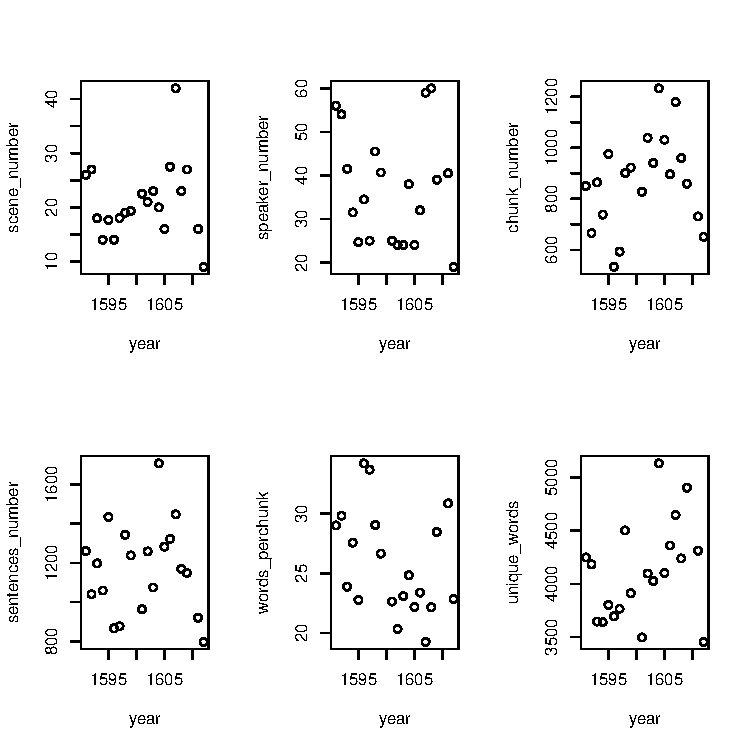
\includegraphics[width=\maxwidth]{figure/r-chunk14-1} 

\end{knitrout}

According to the plot, I guess that number of unique words might be increasing by year in term of statistics. Other elements seems not change with year.
So I use ggplot2 get a clearer view in the sixth plot.

\begin{knitrout}
\definecolor{shadecolor}{rgb}{0.969, 0.969, 0.969}\color{fgcolor}\begin{kframe}
\begin{alltt}
\hlkwd{qplot}\hlstd{(data_sort_byyear[,}\hlnum{1}\hlstd{],data_sort_byyear[,}\hlnum{8}\hlstd{],}\hlkwc{geom}\hlstd{=}\hlkwd{c}\hlstd{(}\hlstr{'point'}\hlstd{,}\hlstr{'smooth'}\hlstd{),}\hlkwc{method}\hlstd{=}\hlstr{'lm'}\hlstd{,}\hlkwc{xlab}
\hlstd{=} \hlstr{'year'}\hlstd{,}\hlkwc{ylab} \hlstd{=} \hlstr{'number of unique words'}\hlstd{)}
\end{alltt}


{\ttfamily\noindent\color{warningcolor}{\#\# Warning: Ignoring unknown parameters: method}}\end{kframe}
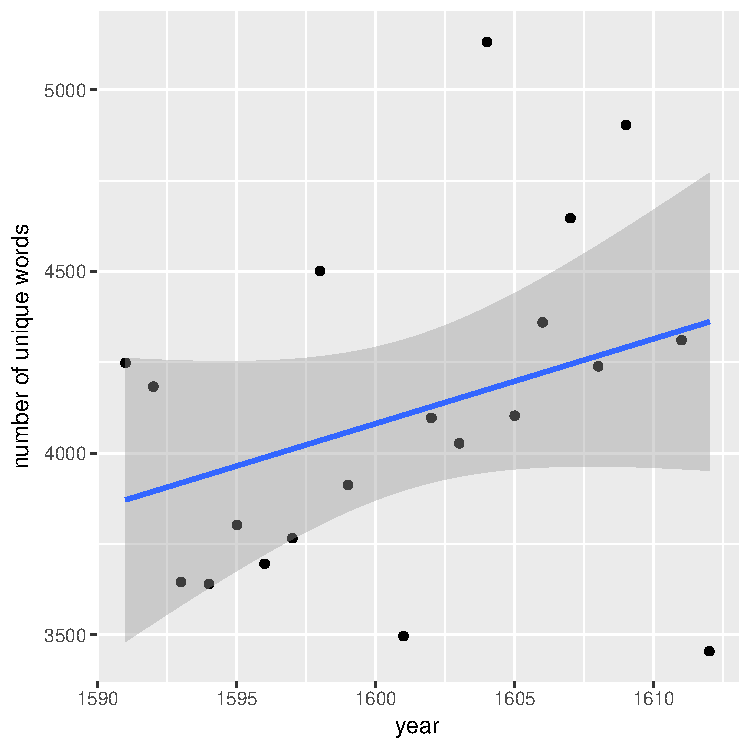
\includegraphics[width=\maxwidth]{figure/r-chunk15-1} 

\end{knitrout}

In addition, I find the p-value is about 0.1 by using lm. So I think unique words increased by year in Shakepeare's play, but the trend is not obvious.

\section{Question 3}

Fields:\\
\quad year='numeric'\qquad year published of the play\\
\quad title='character'\qquad title of the play\\
\quad text='character'\qquad original content of the play\\
\quad body='character' \qquad body of the play\\
\quad chunk='character' \qquad all spoken chunks in the play\\
\quad acts\_number='numeric' \qquad number of acts\\
\quad scenes\_number='numeric' \qquad number of scenes\\
\quad speakers\_number='numeric'\qquad number of unique speakers\\
\quad chunks\_number='numeric' \qquad number of chunks\\
\quad sentences\_number='numeric' \qquad number of sentences\\
\quad words\_number='numeric' \qquad number of total words\\
\quad unique\_words='numeric' \qquad number of unique words\\
\quad words\_perchunk='numeric' \qquad number of words per chunk\\
we can also use prototype to set default of fields except text\\


Methods:\\
in the following methods, input mean the content of methods really need. For example, in method get\_basic\_information, we can input play and use play@text to get text, rather than input text directly.
\\
1.get\_basic\_information : input text of the play and output: year,title,body,acts\_number,scenes\_number \\  
2.get\_chunk : input body of the play and output chunk \\
3.get\_chunk\_information : input chunk and output: speakers\_number,chunks\_number,sentences\_number,words\_number,\\unique\_words,words\_perchunk
  

\end{document}
